\chapter{Robotics}
\marginnote{Needs to be refering more to the project requirements}.

This chapter describes the setup of the robot system, based on the requirements specification. The task of the robot in this project is place the camera sensor at a desired pose. For this purpose a 6 axis Stäubli rx60 has been provided along with a ROS service interface to query and control the configuration. The robot and workcell will be descried in further details in section \ref{sec:robot_physical}. For the robot to be able to move from one pose to another, planners, collision checking and controllers are needed. Since part of the system must run in ROS, it is desired to keep all execution within this framework. It will be assumed in the following, that the reader is familiar with basic ROS terms like nodes, topics, messages, launch files, parameter server, rviz, tf and services, thus only describing MoveIt and ROS control. The recommended approach in that case is to use the MoveIt stack and the ROS control package.  For the planner to be able to do the collision checking without actually colliding, a model of the robot and the workcell must be present. How to setup this model and available parameters are shortly descriped in section \ref{sec:robot_model}. Planning a collision free path is done with ROS MoveIt. ROS Control is used to make the interface between MoveIt and the robot. The MoveIt concepts and how to set it up is described in section \ref{sec:moveit}, a further look in to the planning algorihtms in section \ref{sec:planning} and a short introduction to ROS control in section \ref{sec:robot_control}. A graphical overview of the system is given in figure \ref{fig:workcell_to_moveit_path}

%Leon removed:  used with the focus of making a quick reference for fast setting up a robot system using tool in the ROS framework.

\begin{figure}[htb]
	\begin{center}
		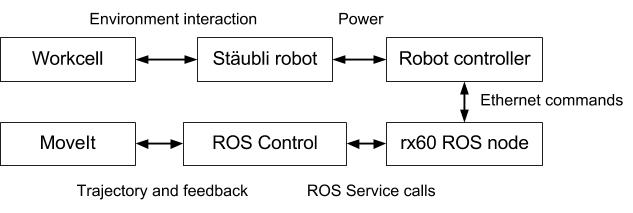
\includegraphics[scale=0.5,trim=0 0 0 0]{graphics/05_robotics/workcell_to_moveIt_path.png}%trim=l b r t
		\caption{Overview of the path from the workcell to the MoveIt stack}
		\label{fig:workcell_to_moveit_path}
	\end{center}
\end{figure}

% Remember to refer the requirement specification, give a breif introduction to why MoveIt has been used and also a short abstact of what this chaper contains. -done, Leon

% General overview of the system

\section{The physical robot and ROS interface}
\label{sec:robot_physical}
% - Staübli (boot up)
The robot provided for this project is a Stäubli RX60b 6 Axis industrial manipulator. When starting the robot a small rotary switch at the bottom of the controller needs to be turned, and after a few minutes the robot will be booted up and ready. Interfacing the robot is done by a small teach pendant, where it is possible to change application, calibrate, manual control etc. For this project a robot application has been provided such that the robot communicates with a ROS node on a provided machine thus almost no interfacing directly with the robot is necessary. When starting the robot it needs to run the robot application, which is done by releasing the emergency stop, pushing the big green button i the top right corner so it lids up and pressing the (un)pause button. When doing tests with the robot it can be recommended to adjust the moving speed to a minimum to avoid accidents. This is done by the plus and minus buttons on the pendant.
% - The tool unit and sensors (breif)
The tool mounted on the tool flange is a 3D printed sensor mount with both a Carmine depth camera and a PointGrey BumbleBee stereo camera. Wires have been strip mounted to the robot to avoid them getting stuck in the moving parts. 
% - Workcell
The workcell contains the robot placed on a plane big surface, a Troax safety fence and a radiator. Both the fence and the radiator is placed in such distance that the robot will only be able to collide with them in very few configurations. The workcell can be seen in figure \ref{fig:workcell} \marginnote{Image placeholder}.

\begin{figure}[htb]
	\begin{center}
		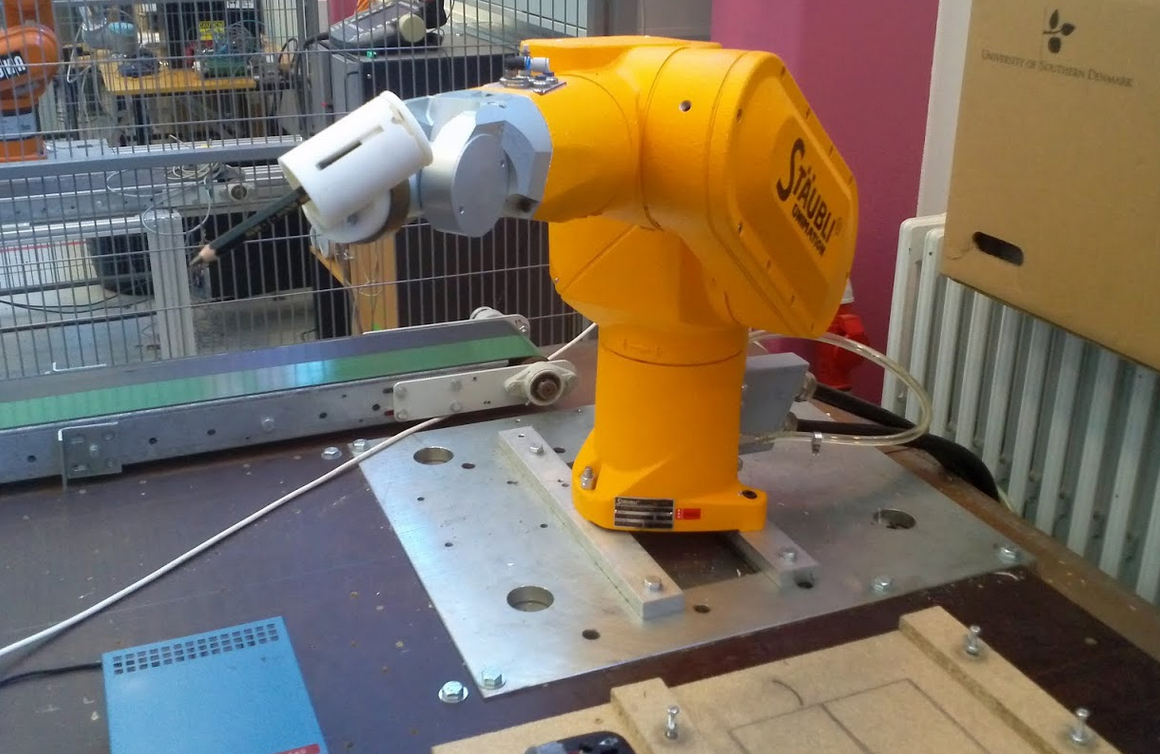
\includegraphics[scale=0.4,trim=0 0 0 0]{graphics/05_robotics/workcell.png}%trim=l b r t
		\caption{Picture of the workcell}
		\label{fig:workcell}
	\end{center}
\end{figure}


% ------------------------------------------- PICTURE OF ROBOT AND WORKCELL ---------------------------------------

% - The ROS service interface
The robot axis are controlled by the robot controller which are then connected to a computer with a provided ROS application for communication. To control the robot service calls needs to be made to this node. These service calls provides functionality such as setting various limits, tool position, valve control and most important joint configurations. Furthermore it allows values to be read from the robot, such that feedback can be supplied to the trajectory controller.

\section{Robot model}
\label{sec:robot_model}
To be able to plan a trajectory for the robot, the planner needs a model of the robot. This model is used for kinematics but also to avoid self collision. The format for describing a robot in ROS is Unified Robot Description Format (URDF). It is also possible to define the robot in the XACRO macro format and convert it to the macro language URDF, however in this project the robot has been descried directly in URDF.
% - URDF format and tools (can also be used in gazebo)
A tool that can be used to generate the URDF file directly from a CAD assembly file is available under the name "SolidWorks to URDF Exporter". This tool was used as a basis for the URDF file for this project, but the quality of the output is somehow questionable. A RobWork workcell containing the description of the RX60 robot was available for the project and has been used as a reference to describe the joints, joints limits and also as source for robot CAD files. It needs to be noticed that CAD format has to be binary STL to work as part of the robot description. The tool on the robot has also been described in the URDF to give the necessary transforms for the camera sensors and a intuitive looking visualization of the robot. In the URDF file it is possible to define both a visual CAD of the joints but also a CAD only used for collision checking. To be sure that the tool does not collide with anything, the collision model is a large box with a least 10mm extra space margin with respect to the visual model. The model can be seen on figure \ref{fig:tool_collision_model}. To use the URDF file it has to be put into the ROS parameter server which can be done in the launch file.

\begin{figure}[htb]
	\begin{center}
		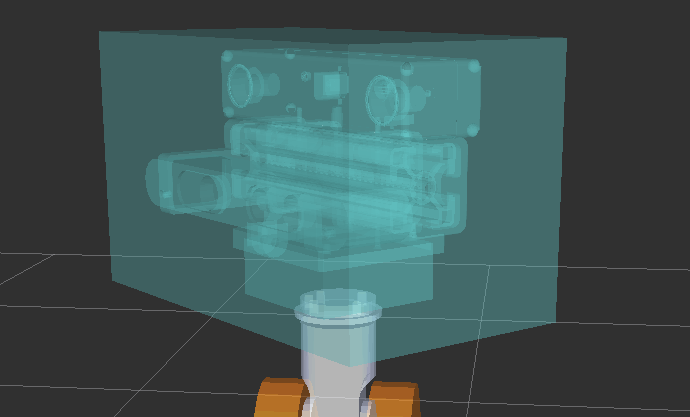
\includegraphics[scale=0.5,trim=0 0 0 0]{graphics/05_robotics/tool_collision_model.png}%trim=l b r t
		\caption{The tool mounted on the robot flange and the collision model shown in transparent}
		\label{fig:tool_collision_model}
	\end{center}
\end{figure}

% - - Collision model and visual model
% - TF tree
% - Visualization
\section{ROS MoveIt}
\label{sec:moveit}
ROS MoveIt is a software planing tool that collect many open source libraries into a tool that can easily be used for planning with both simple and high dimensionality robots.  Controlling a robot with MoveIt can be done in the C++ or python, but it also features a planning plug-in for the ROS visualizer (Rviz). Combining the programming interface with Rviz gives a great visual feedback, where the planned trajectory can be visualized before and while moving the robot as seen on figure \ref{fig:robot_trajectory}.

%Leon removed: A great example of a complex robot is the PR2 robot developed at Willow Garage that runs on MoveIt.

\begin{figure}[htb]
	\begin{center}
		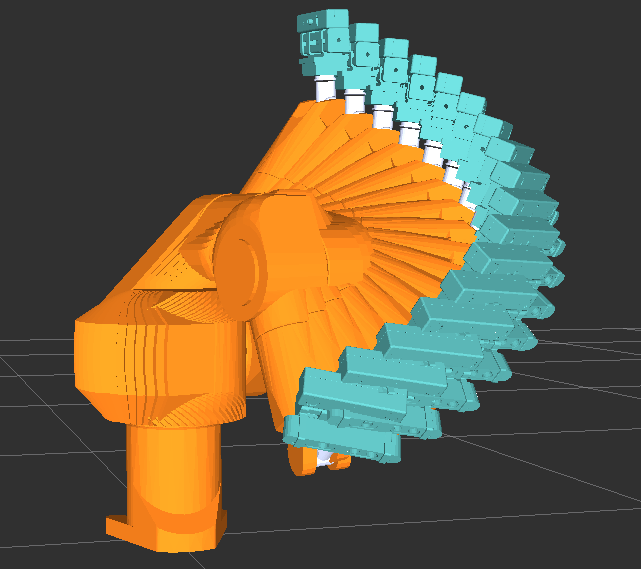
\includegraphics[scale=0.5,trim=0 0 0 0]{graphics/05_robotics/robot_trajectory.png}%trim=l b r t
		\caption{Robot trajectory displayed as a series of robot configurations in Rviz}
		\label{fig:robot_trajectory}
	\end{center}
\end{figure}

When planning in MoveIt it will by default use the Open Motion Planneing Library (OMPL), however MoveIt provides a plugin interface allowing custom planners to be used. OMPL is a collection of state of art sample based planners that takes a planning request and collision detector as input and if successful returns a planned path. MoveIt then generate a trajectory from the path according to the given robot constraints. The collision checking in MoveIt is done by Flexible Collision Library (FCL). This collision detection allows different input models, such as robot self-collision, workcell model collision and collision with sensed objects. For collision with sensed data, MoveIt has a self-filter, such that if a part of the robot is sensed it can be filtered away from collision map. Without this feature, the sensed robot would collide with the kinematic calculated position of the robot. When configuring a robot with MoveIt a Allowed Collision Matrix (ACM) is generated. This matrix defines joints on the robot that do not need to be checked for collision, such as joints that may never collide in any configuration and succeeding joints. Succeeding joints are of cause able to collide, but this should be avoided by setting prober joint movement constraints instead of the collision detector, as a collision detection calls are expensive in computation. As default MoveIt uses Orocos Kinematics and Dynamics(KDL) for solving the kinematics. MoveIt contains a setup tool, MoveIt Setup Assistant (figure \ref{fig:moveit_setup_assistant}) with a guide trough the whole set up process.

%Leon removed: , but for complex robots it is recommended to compile a robot specific solver using OpenRave IKfast. The advantage of a IKfast compiled solver is that it is able to use analytical solvers instead of numerical. ; When the model of the robot is present, it is easy to start using MoveIt. 

\begin{figure}[htb]
	\begin{center}
		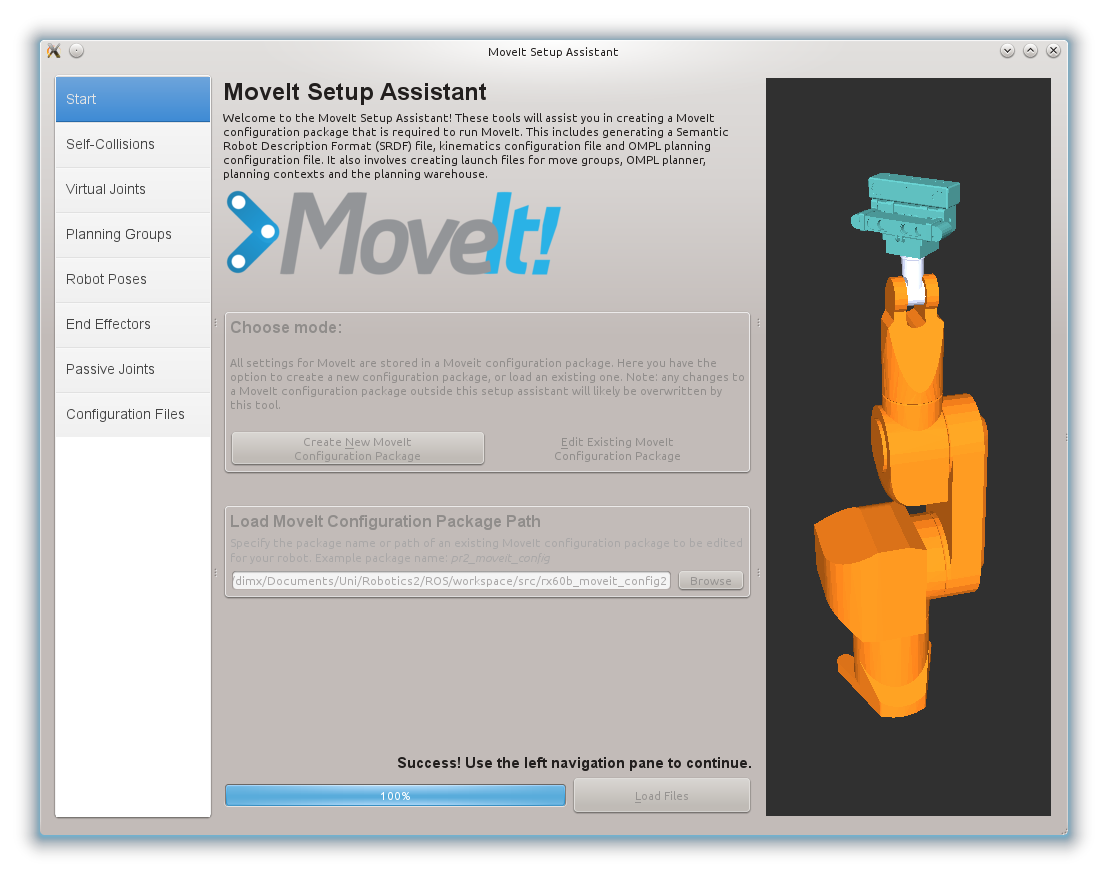
\includegraphics[scale=0.4,trim=0 0 0 0]{graphics/05_robotics/moveit_setup_assistant.png}%trim=l b r t
		\caption{The MoveIt setup tool}
		\label{fig:moveit_setup_assistant}
	\end{center}
\end{figure}

When the MoveIt setup tool has been run, a ROS package has been generated with the proper launch files to start planning with the robot. This package features a demo application which launches Rviz with the motion plugin, so the robot can be seen running. For the real robot to move, at least one controller needs to be implemented. This is described in section \ref{sec:robot_control}.

% - Features / introduction
% - - Support for octomap input for collsion checking with self-filter (removes visible parts of the robot from the map)
% - - OMPL - Motion planning (OMPL itself has no concept of a robot)
% - - OpenRave IKFast - Kinematic solver / Orocos KDL
% - - FCL - Collision checking
% - Importing the robot (robot setup tool)
% - Interfaces (rviz, c++, trajectory service)
% - - rviz, c++
% - - controller manager (trajectory action interface)
% - Constrainting the robot

% - Robot state publisher (TF)


\section{Planning}
\label{sec:planning}
% ------------ Things that we have been discussing in class do not need to be described in very fine detail -----------

Tough many planners are available in the OMPL, it has been chosen to use Probabilistic RoadMap (PRM) \marginnote{OMPL har tre forskellige: geometric, geometric lazy og geometric PRMstar. Hvilken bruger vi?}for this project. PRM is a probabilistic complete multi query planning algorithm with two phases. First the learning phase generates roadmaps in the configuration space by random sampling and collision checking, next the query phase is used to connect the start and goal configuration to the roadmap and within the roadmap find a valid path. The PRM planner has been chosen because the work cell is static and thus the roadmap can be generated beforehand to speed up the planning requests. Which planner to use in MoveIt is defined in the planning request to allow the use of specific planners for specific tasks.

\marginnote{Vi har intet om optimisation...}

% --- BRING UP SOME CODE FROM OMPL!


% - PRM planner
% - Path optimization
% - How is it done in OMPL?
% -- Static work space
% -- All types of problems, many DOF
% -- learning phase, query phase


\section{Robot control}
\label{sec:robot_control}
% - ROS Control framework
When MoveIt has generated a trajectory for the robot, a controller needs to take care of the physical movement. In the package generated by MoveIt the control is done by fake\_controller which does not actually control anything. First of all the MoveItSimpleControllerManger needs to be loaded to provide a service interface for the actual controller. For actual control there is a package called ros\_control which provides a framework and tools for implementing a robot controller. The ros\_control package consists of a controller manager, a hardware\_interface and different types of controllers. To get the robot running, a new package with a node for the controller has to be made. In the node, the framework is included and a description of the robot inputs and outputs are defined. The control loop of the node fetches the state from the robot and passes this to the controller. The controller then outputs the desired movement for the robot which has to be passed on to the robot. As described in section \ref{sec:robot_physical} the interfacing to the physical robot is done by service calls. In the project it has been chosen that the controller node also is responsible of publishing the current robot state. The robot state is used by MoveIt and robot\_state\_publisher. The robot\_state\_publisher is the node responsible for updating the TF tree. 


% Action and service interfaces
% The action controller in moveit
% the fake_controller in moveit
% joint_state_publisher


%Motion planning
%  general motion planning, kinematics
%  Available tools in ROS
%  MoveIt planner concepts
%  Setting up a new robot with MoveIt
%  Robot model (URDF (joints, links, limits, transforms) , CAD, rviz/TF)
%Robot controller
%
%C++ planning interface
